%!TEX root = ../main.tex
% chktex-file 46
\chapter{Learning to Aggregate on Graphs}%
\label{sec:ltag}

In the previous chapter an introduction to two separate fields of research was given:
\begin{enumerate*}
	\item \Acf{lta},
	\item \Acf{gcr}
\end{enumerate*}.
In this chapter we will combine them and define an extension of \ac{lta} to the \ac{gcr} problem.
This will be done in three steps:
\begin{enumerate}
	\item We begin with a formal definition of what actually constitutes an \ac{lta} method as opposed to non-\acs{lta} methods.
	\item Using this definition, we will see that some of the previously described \ac{gcr} methods can be interpreted as \ac{lta} variants under certain conditions.
	\item Finally a novel \acs{lta}-inspired \ac{gcnn} architecture will be described.
\end{enumerate}

\section{A Generalized Definition of \acs*{lta}}%
\label{sec:ltag:definition}

In order to formally define \ac{lta}, we must first decide on its defining characteristic.
We propose that this characteristic should be the \textit{localized explainability} of \ac{lta} predictions.
As seen in \cref{sec:related:lta}, an \ac{lta} score $y_{C} \in \mathcal{Y}$ for some multiset composition $C = \ldblbrace c_1, \dots, c_n \rdblbrace$ can always be tracked back to a set of local constituent scores $y_1, \dots, y_n \in \mathcal{Y}$.
Under the assumption that each constituent $c_i$ represents some human interpretable object, a composition's score $y_{C}$ can therefore be explained by the presence of certain indicative constituents/objects $c_i$.

Based on this intuition we now give a generalized definition of \ac{lta} which applies to unstructured as well as structured input data.
We assume that all compositions are represented by graphs $G \in \mathcal{G}$;
an unstructured input is represented by a graph with one vertex per constituent ($\mathcal{V}_G = \{ v_{c_1}, \dots, v_{c_n} \}$) and no edges ($\mathcal{E}_G = \emptyset$).
Each composition has some target score $y_G \in \mathcal{Y}$ which could be a discrete class or continuous value.
An \textit{\ac{lta} model} $h: \mathcal{G} \to \mathcal{Y}$ assigns predictions $\hat{y}_G \in \mathcal{Y}$ to compositions $G$ which ideally correspond to the true score $y_G$.
Such a model must satisfy three criteria:
\begin{enumerate}[label=\textbf{\arabic*.}]
	\item \textbf{Decomposition:}
		A given composition $G$ must be decomposed into a set of constituents $c_{G,i}$ via a \textit{decomposition function} $\psi: \mathcal{G} \to \mathcal{P}(\mathcal{G})$.
		\begin{defn}\label{defn:ltag:decomp}
			$\psi$ is a \textit{decomposition function} iff.\ it splits a graph into a subset of its subgraphs, i.e.\ $\forall G \in \mathcal{G}: \forall c_{G,i} \in \psi(G): \exists s \in \mathcal{P}(\mathcal{V}_G): c_{G,i} = G[s]$.
		\end{defn}
		Note that the strict equality $c_{G,i} = G[s]$ is used in \cref{defn:ltag:decomp} instead of just requiring subgraph isomorphism ($c_{G,i} \simeq G[s]$) because a constituent $c_{G,i}$ represents a specific localized subgraph of a structured composition.

		In the existing unstructured \ac{lta} approaches the decomposition function is implicitly defined as $\psi(G) \coloneqq {\{ G[v_{c_i}] \}}_{v_{c_i} \in \mathcal{V}_G}$ since each vertex $v_{c_i}$ corresponds to an interpretable constituent $c_i$ by definition.
		For structured data however, a split into individual vertices is typically not appropriate.
		Molecular graphs from chemical datasets for example are meaningfully characterized by the presence of so-called \textit{functional groups} consisting of multiple bonded atoms while a characterization on the level of individual atoms is generally less meaningful~\cite{McNaught1997}.
	\item \textbf{Local evaluation:}
		The constituents $c_{G, i} \in \psi(G)$ must be evaluated via some function $f: \mathcal{G} \to \mathcal{Y} \times \mathbb{R}$.
		This \textit{evaluation function} assigns a prediction $\hat{y}_{G, i} \in \mathcal{Y}$ and a weight $w_{G, i} \in \mathbb{R}$ to each constituent.
		A constituent's weight $w_{G, i}$ can intuitively be interpreted as a measure of the confidence that the local prediction $\hat{y}_{G, i}$ is indicative of the composition's global target score $y_G$.
		Learning local predictions and weights for all possible constituents is called the \textit{disaggregation problem}.

		Note that there are no explicit constituent weights in the existing unstructured \ac{lta} approaches (i.e.\ implicitly all $w_{G, i} = 1$) because the explicitly given constituents are assumed to be equally indicative of $y_G$.
		For structured data however, where the decomposition $\psi(G)$ is not given as part of the input, this assumption does not necessarily hold.
		By weighting the constituents, an \ac{lta} model can reduce the relevance or even ignore constituents that turn out to be irrelevant for the compositions target score $y_G$.
	\item \textbf{Aggregation:}
		Lastly a \textit{weighted aggregation function} $\mathcal{A}: {(\mathcal{Y} \times \mathbb{R}_{\geq 0})}^{*} \to \mathcal{Y}$ must be applied.
		It combines the multiset of local constituent predictions and non-negative weights into a single global composition prediction.
		\begin{defn}\label{defn:ltag:weighted-agg}
			We call $\mathcal{A}$ a \textit{weighted aggregation function} iff.\ it satisfies
			\begin{align*}
				\text{idempotency: } & \exists \eta > 0: \forall y \in \mathcal{Y}, w \in \mathbb{R}_{\geq 0}^n\text{ s.t. }{\max w} \geq \eta: \mathcal{A}({\ldblbrace (y, w_i) \rdblbrace}_{i=1}^n) = y \\
				\land\text{ zero invar.: } & \forall y_0 \in \mathcal{Y}, S = {\ldblbrace (y_i, w_i) \rdblbrace}_{i=1}^n: \mathcal{A}(S \cup \{ (y_0, 0) \}) = \mathcal{A}(S) \text{.}
			\end{align*}
		\end{defn}
		{\setlength{\parskip}{0pt}The idempotency constraint requires aggregation functions to agree with uniform input scores $y$ if at least one input is weighted above some threshold $\eta$.
		The zero invariance constraint requires aggregation functions to ignore inputs with zero weight.
		Exemplary weighted aggregation function are:}
		\begin{itemize}
			\item The \textit{weighted mean} function $\wmean({\ldblbrace (y_i, w_i) \rdblbrace}_{i=1}^n) \coloneqq \sum_{i=1}^n w_i y_i$ which requires $\sum w_i = 1$, $w_i \in [0, 1]$ and the existence of some scalar multiplication operator $\cdot: \mathbb{R} \times \mathcal{Y} \to \mathcal{Y}$, typically from some subfield $\mathcal{Y} \subseteq \mathbb{R}$ or possibly also some vector subspace $\mathcal{Y} \subseteq \mathbb{R}^d$.
			\item Another basic weighted aggregator is the \textit{weighted majority vote} function $\wmaj({\ldblbrace (y_i, w_i) \rdblbrace}_{i=1}^n) \coloneqq {\arg\max}_{y \in \mathcal{Y}} \sum_{y_i = y} w_i$ which returns the input with the highest total weight.
				Unlike $\wmean$ it can also be applied to score domains $\mathcal{Y}$ without a multiplication operator, e.g.\ sets of discrete classes.
			\item Alternatively an unweighted aggregation function like $\min$, $\max$, $\mean$ or \ac{owa}\footnote{
				Even though \ac{owa} uses weights, it does not get those weights as part of the input and is therefore considered to be unweighted in this context.
			} also trivially satisfies \cref{defn:ltag:weighted-agg} if all inputs $y_i$ with $w_i = 0$ are filtered out and the weights for all remaining inputs are ignored.
		\end{itemize}
\end{enumerate}
\begin{figure}[ht]
	\centering
	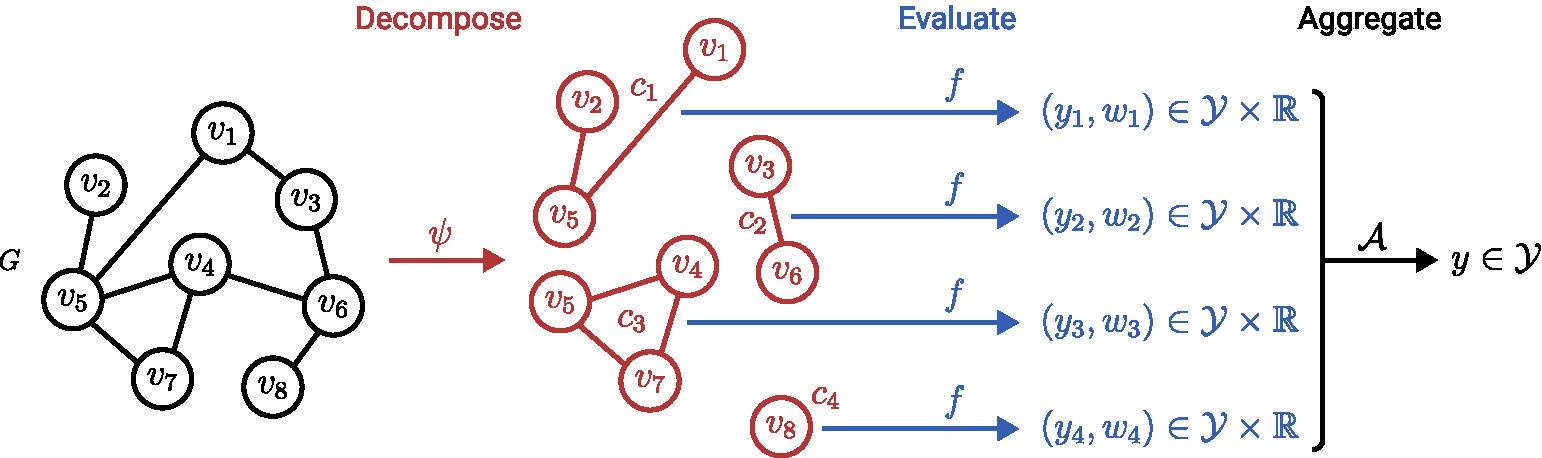
\includegraphics[width=\linewidth]{gfx/graph-lta/ltag-overview.pdf}
	\caption{
		Overview of the generalized \ac{lta} architecture for structured data.
	}\label{fig:ltag:ltag-overview}
\end{figure}
Based on the notion of decomposition, local evaluation and aggregation we can now define the concept of \textit{\ac{lta} formulations}.
\begin{defn}
	A model $h: \mathcal{G} \to \mathcal{Y}$ is in an \textit{\ac{lta} formulation} iff.\ it is expressed as
	\begin{align*}
		h(G) \coloneqq \mathcal{A}(\ldblbrace f(c_{G,i})\, |\, c_{G,i} \in \psi(G) \rdblbrace) \quad\text{with $\psi$, $f$ and $\mathcal{A}$ as defined above.}
	\end{align*}
\end{defn}
Note that every model $h: \mathcal{G} \to \mathcal{Y}$ has a trivial recursive \ac{lta} formulation by choosing $\psi(G) = \{ G \}$, $f(G) = (h(G), 1)$ and an arbitrary weighted aggregation function $\mathcal{A}$.
Those trivial \ac{lta} formulations do not split compositions into locally evaluated constituents and therefore intuitively do not fulfill the postulated localized explainability characteristic of \ac{lta}.
However since there is no commonly accepted formal criterion to decide whether a model's decisions are explainable~\cite{Lipton2018}, we do not attempt to strictly distinguish between \ac{lta} and non-\acs{lta} methods.
Instead the notion of \ac{lta} formulations should be seen as way to identify how ``\acs{lta}-like'' a model is:
\begin{itemize}
	\item \textbf{Negative extreme:}
		If a model $h$ only has trivial \ac{lta} formulations with the decomposition function $\psi(G) = \{ G \}$, it is not considered to be an \ac{lta} model.
	\item \textbf{Positive extreme:}
		If a model has an \ac{lta} formulation with a decomposition function that returns interpretable constituents, it is considered to be an \ac{lta} model.
		By definition this is true for the single-vertex constituents $\psi(G) \coloneqq {\{ G[v_{c_i}] \}}_{v_{c_i} \in \mathcal{V}_G}$ of \ac{lta} methods for unstructured data.
	\item \textbf{In-between cases:}
		An \ac{lta} method for structured data must produce models that lie somewhere in-between the two extremes.
\end{itemize}

The more ``\acs{lta}-like'' a given model is, the stronger its bias towards locally explainable predictions, which in turn reduces the potential expressive power of the model.
\citet{Gilpin2018} describe this trade-off between explainability and expressive power in more detail.
However, when considering problem domains in which the true composition scores $y_G$ are accurately described by an \acs{lta}-like generative process, a less expressive \ac{lta}-like model could generalize better than a more expressive non-\ac{lta} model.
This idea is captured by the so-called \textit{\ac{lta} assumption}.
\begin{defn}
	A problem domain $\mathcal{D}$ satisfies the \textit{\ac{lta} assumption} iff.\ there is an \ac{lta} method which produces models with an equal or lower out-of-sample error than the models produced by non-\acs{lta} methods for most training samples $\mathcal{D}_{\text{train}} \subseteq \mathcal{D}$.
\end{defn}
Due to the fuzziness of the class of \ac{lta} methods, the \ac{lta} assumption is naturally also a fuzzy concept.
Nonetheless evidence for its truthiness in a given domain $\mathcal{D}$ can be empirically obtained by comparing candidate \ac{lta} methods with the best known non-\ac{lta} method for $\mathcal{D}$, assuming that some cut-off condition for the required ``\ac{lta}-ness'' of an \ac{lta} method is agreed upon.

\section{\acs*{lta} Formulations of Existing \acs*{gcr} Methods}%
\label{sec:ltag:formulation}

Based on the general definition of \ac{lta} from the last section, we will now see to what extent the \ac{gcr} methods described in \cref{sec:related:gcr} can be interpreted as \ac{lta} instances.
First the relation between \acp{svm} on graph embeddings and \ac{lta} will be explored.
Then we will provide an \ac{lta} perspective on \acp{gcnn}.

\subsection{\acsp*{svm} using Graph Embeddings as \acs*{lta} Models}%
\label{sec:ltag:formulation:svm}

In \cref{sec:related:gcr:embed,sec:related:gcr:kernel} three different ways to map a given graph $G$ to a vector $\varphi(G) \in \mathbb{R}^d$ were described:
\begin{enumerate*}
	\item Fingerprint embeddings,
	\item skip-gram inspired embeddings and
	\item kernel embeddings
\end{enumerate*}.
One common way to solve the \ac{gcr} problem via those embedding vectors is to train an \ac{svm} on them.
We will now see that \acp{svm} can be interpreted as \ac{lta} models if they are trained on so-called \acp*{sce}.
\begin{defn}
	Given a a multiset $A = \ldblbrace \underbrace{a_1, \dots, a_1}_{\gamma_A(a_1)\text{ times}},\allowbreak \dots, \underbrace{a_n, \dots, a_n}_{\gamma_A(a_n)\text{ times}} \rdblbrace \subseteq D$, the so-called \textit{multiplicity function} $\gamma_A: D \to \mathbb{N}_0$ maps each element of the domain $D$ to its multiplicity in $A$ with $\gamma_A(x) = 0 \Leftrightarrow x \notin A$.
\end{defn}
\begin{defn}\label{defn:ltag:substruct-embedding}
	A graph embedding $\varphi: \mathcal{G} \to \mathbb{N}_0^{d}$ is called a \ac{sce} iff.\ %
	there are decomposition functions $\psi_{\varphi, i}: \mathcal{G} \to \mathcal{P}(\mathcal{G})$ and multiplicity functions $\gamma_{\varphi, i}: \mathcal{G} \to \mathbb{N}_0$ for all embedding components $i \in [d]$ s.t.\ %
	$\forall G \in \mathcal{G}, i \in [d]: \varphi(G)[i] = \sum_{c \in \psi_{\varphi, i}(G)} \gamma_{\varphi, i}(c)$ where $\gamma_{\varphi, i}$ is the multiplicity function of a multiset of the constituents $\psi_{\varphi, i}(G)$.
	We call $\psi_{\varphi, i}$ an \textit{underlying decomposition} of the $i$-th component of the embedding $\varphi$.
	Similarly the joint decomposition $\psi_{\varphi}(G) \coloneqq \bigcup_{i=1}^d \psi_{\varphi,i}(G)$ is an \textit{underlying decomposition} of $\varphi$.
\end{defn}
Intuitively \cref{defn:ltag:substruct-embedding} states that the value of each \ac{sce} component must be derived from the number of constituents produced by some decomposition function where each constituent might be counted multiple times.
Based on this requirement we now proof the main theorem which shows the relation between \acp{svm} and \ac{lta}.

\begin{thm}\label{thm:ltag:svm-ltag-formulation}
	A binary \ac{svm} graph classifier $h$ that applies a \ac{sce} $\varphi$ to its inputs has an \ac{lta} formulation that uses an underlying decomposition $\psi_{\varphi}$ of $\varphi$.
\end{thm}
\begin{proof}
	Let $h: \mathcal{G} \to {\{ -1, +1 \}}$ be a binary graph classifier expressed as $h = h_{\text{\acs*{svm}}} \circ \varphi$ where $\varphi: \mathcal{G} \to \mathbb{N}_0^{d}$ is an \ac{sce} and $h_{\text{\acs*{svm}}}: \mathbb{R}^{d} \to {\{ -1, +1 \}}$ a standard \ac{svm} classifier.
	Additionally, let $\psi_{\varphi}$ be some underlying decomposition of $\varphi$ with ${\{ \gamma_{\varphi, i} \}}_{i=1}^d$ being the corresponding multiplicity functions.

	Based on this decomposition we now bring the \ac{svm} graph classifier $h$ into an \ac{lta} formulation.
	If $h$ is trained on a dataset $\mathcal{D}_{\text{train}} = {\{ (G_1, y_1), \dots, (G_N, y_N) \}}$, via the kernel trick it can be expressed as
	\begin{align*}
		h(G) &= \sgn\left( \sum_{j = 1}^{N} \alpha_j y_j {\langle \varphi(G), \varphi(G_j) \rangle} + b \right)
		\quad\text{for some $\alpha \in \mathbb{R}_{\geq 0}^N$ and $b \in \mathbb{R}$} \\
		&= \sgn\left( {\sum_{i=1}^{d} {
				\varphi(G)[i]
				\underbrace{\left( \sum_{j = 1}^{N} \alpha_j y_j {\varphi(G_j)}[i] \right)}_{\beta_i}}
			} + b \right)
		 = \sgn\left( {\sum_{i=1}^{d} \varphi(G)[i] \beta_i} + b \right) \\
		&= \sgn\left( {\sum_{c_t \in \psi_{\varphi}(G)} \underbrace{\sum_{i = 1}^d \gamma_{\varphi, i}(c_t) \beta_i}_{z_t}} + b \right)
		 = \sgn\left( {\sum_{c_t \in \psi_{\varphi}(G)}} \underbrace{|z_t|}_{w_t} \underbrace{\sgn{z_t}}_{y_t} + {\underbrace{|b|}_{w_b} \underbrace{\sgn{b}}_{y_b}} \right) \\
		&= \wmaj\left( \ldblbrace (y_t, w_t)\, |\, c_t \in \psi_{\varphi}(G) \rdblbrace \cup \ldblbrace (y_b, w_b) \rdblbrace \right)
		\text{.}
	\end{align*}
	By choosing $f_h(c_t) \coloneqq (y_t, w_t)$ and $\mathcal{A}_h(S) = \wmaj(S \cup \ldblbrace (y_b, w_b) \rdblbrace)$, the \ac{svm} model therefore has an \ac{lta} formulation with the decomposition function $\psi_{\varphi}$.

	To complete the proof it now remains to show that $f_h$ and $\mathcal{A}_h$ are in fact a local evaluation function and a weighted aggregation function respectively.
	To see that $f_h$ perform local evaluation, note that $f_h(c_t) \coloneqq (\sgn z_t, {|z_t|})$ with $z_t \coloneqq \sum_{i=1}^{d} \gamma_{\varphi,i}(c_t) \beta_i$ only depends on the shared multiplicity functions $\gamma_{\varphi,i}$, the constants $\beta_i$ and the constituent $c_t$;
	apart from $c_t$ no other information from the input graph $G$ is required by $f_h$ which makes it a local evaluation function.
	To see why $\mathcal{A}_h$ satisfies \cref{defn:ltag:weighted-agg}, note that it inherits the idempotency property from $\wmaj$ because $\mathcal{A}_h$ ignores the bias ``pseudo-constituent'' $(y_b, w_b)$ for all threshold weights $\max w_t \geq \eta > w_b$, similarly the zero invariance of $\wmaj$ is also directly inherited.
	This concludes the proof.
\end{proof}

The central statement of \cref{thm:ltag:svm-ltag-formulation} is that \acs{svm} graph classifiers that use an \ac{sce} $\varphi$ implicitly perform an \acs{lta}-like weighted majority vote aggregation of constituent scores $y_t$.
Those constituent scores can in turn be expressed as a majority vote of the graph scores in the training dataset $\mathcal{D}_{\text{train}}$:
\begin{align}
	y_t \coloneqq \sgn z_t
	 &= \sgn\left( \sum_{j=1}^N \underbrace{\left( \alpha_j \smashoperator[l]{\sum_{c_k \in \psi_{\varphi}(G_j)}} \sum_{i=1}^d \gamma_{\varphi,i}(c_t) \gamma_{\varphi,i}(c_k) \right)}_{w_j \geq 0} y_j \right) \\
	 &= \wmaj(\ldblbrace (y_j, w_j)\, |\, j \in [N] \rdblbrace) \nonumber
\end{align}
Note that, if the constituents of $G_j$ all come from different embedding components than those of $G$ ($\forall i \in [d]: {\psi_{\varphi, i}(G_j) \cap \psi_{\varphi, i}(G)} = \emptyset$), then $G_j$ has no influence on the score of $G$ ($w_j = 0$).

To see what \cref{thm:ltag:svm-ltag-formulation} implies in practice, we will now apply it to the graph embedding approaches described in \cref{sec:related:gcr:embed,sec:related:gcr:kernel}:
\begin{enumerate}[label=\textbf{\arabic*.},ref={\arabic*}]
	\item \textbf{Fingerprint embeddings:}\label{itm:ltag:fingerprint-lta-formulation}
		Here the $i$-th embedding component represent the number of occurrences of a substructure $S_i$, i.e.\ ${\varphi}_{\text{FP}}(G)[i] \coloneqq \mathit{count}_{S_i}(G)$ (see \cfullref{defn:related:wl-count-detect}).
		Such a fingerprint embedding naturally is an \ac{sce} with the decomposition functions $\psi_{\text{FP}, i}(G) \coloneqq \{ G[\set(s)]\, |\, s \in \mathcal{V}_G^{*} \land G[s] \equiv S_i \}$ and the multiplicity functions $\gamma_{\text{FP}, i}(c) \coloneqq \mathbbm{1}[c \simeq S_i]$ since those functions produce the subgraphs that are counted by ${\varphi}_{\text{FP}}(G)[i]$ with multiplicity $1$. % chktex 21

		Under the assumption that the substructure patterns $S_i$ are chosen s.t.\ the their instances $c \in \psi_{\text{FP}, i}(G)$ are nontrivial interpretable constituents, the underlying joint decomposition $\psi_{\text{FP}}(G) \coloneqq \bigcup_{i=1}^d \psi_{\text{FP}, i}(G)$ must also be nontrivial and interpretable.
		Thus, by \cref{thm:ltag:svm-ltag-formulation}, \acp{svm} trained on fingerprint embeddings are \ac{lta} models that produce locally explainable predictions.
		\badgebox[t_green]{\acs*{lta}}
	\item \textbf{\texttt{graph2vec}:}
		The skip-gram inspired \texttt{graph2vec} embedding produces vectors $\varphi(G) \in \mathbb{R}^d$ whose individual components do not have a clear interpretation.
		\texttt{graph2vec} embeds graphs that have common 1-\acs{wl} colors closer to each other than graphs that do not share the same colors (see \cfullref{eq:related:graph2vec}).
		The resulting component values can be arbitrary reals, therefore this approach is not an \ac{sce} which in turn implies that it does not have an \ac{lta} formulation as in \cref{thm:ltag:svm-ltag-formulation}.
		\badgebox[t_red]{non-\acs*{lta}}
	\item \textbf{\ac{wl} subtree kernel:}\label{itm:ltag:wlst-lta-formulation}
		The individual components of the \ac{wl} subtree kernel's embedding $\varphi_{\text{ST}}$ represent the number of occurrences of a color $\kappa_i \in \mathcal{C}$, i.e.\ $\varphi_{\text{ST}}(G)[i, t] \coloneqq \mathit{dist}_{\chi_{G,1}^{(t)}}(\kappa_i)$ as defined in \cfullref[ on ]{eq:related:wl-subtree-kernel}\footnote{
			To avoid confusion $\kappa_i \in \mathcal{C}$ is used for colors and $c_j \in \mathcal{G}$ for constituents in this context.
		}.
		The occurrence of a color $\kappa_i$ at some vertex $v_j \in \mathcal{V}_G$ in the $t$-th refinement step (i.e.\ $\chi_{G,1}^{(t)}(v_j) = \kappa_i$) in turn implies that the \ac{bfs} tree $S_{j,t} \coloneqq \text{\acs*{bfs}}(G, v_j, t)$ of depth $t$ rooted at $v_j$ is isomorphic to some \ac{wl} color subtree $S_{\kappa_i}$ (i.e.\ $S_{j,t} \simeq S_{\kappa_i}$).
		This relation between \ac{wl} colors $\kappa_i$ and subtrees $S_{\kappa_i}$ was illustrated in \cfullref[ on ]{fig:related:wl-subtree}.

		To show that $\varphi_{\text{ST}}$ is an \ac{sce}, we have to define decomposition functions $\psi_{\varphi, i, t}$ and multiplicity functions $\gamma_{\varphi, i, t}$ s.t.\ $\varphi(G)[i, t] = \sum_{c \in \psi_{\varphi, i, t}(G)} \gamma_{\varphi, i, t}(c)$.
		Since $\varphi(G)[i, t]$ counts the occurrences $S_{j,t}$ of a subtree $S_{\kappa_i}$ in $G$, the \ac{sce} requirement would be trivially satisfied if each $S_{j,t}$ were a constituent with multiplicity $1$.
		This intuition is however not quite correct because the constituents of a graph $G$ must be induced subgraphs of $G$, not \ac{bfs} subtrees $S_{j, t}$ of $G$.
		\begin{figure}[t]
			\centering
			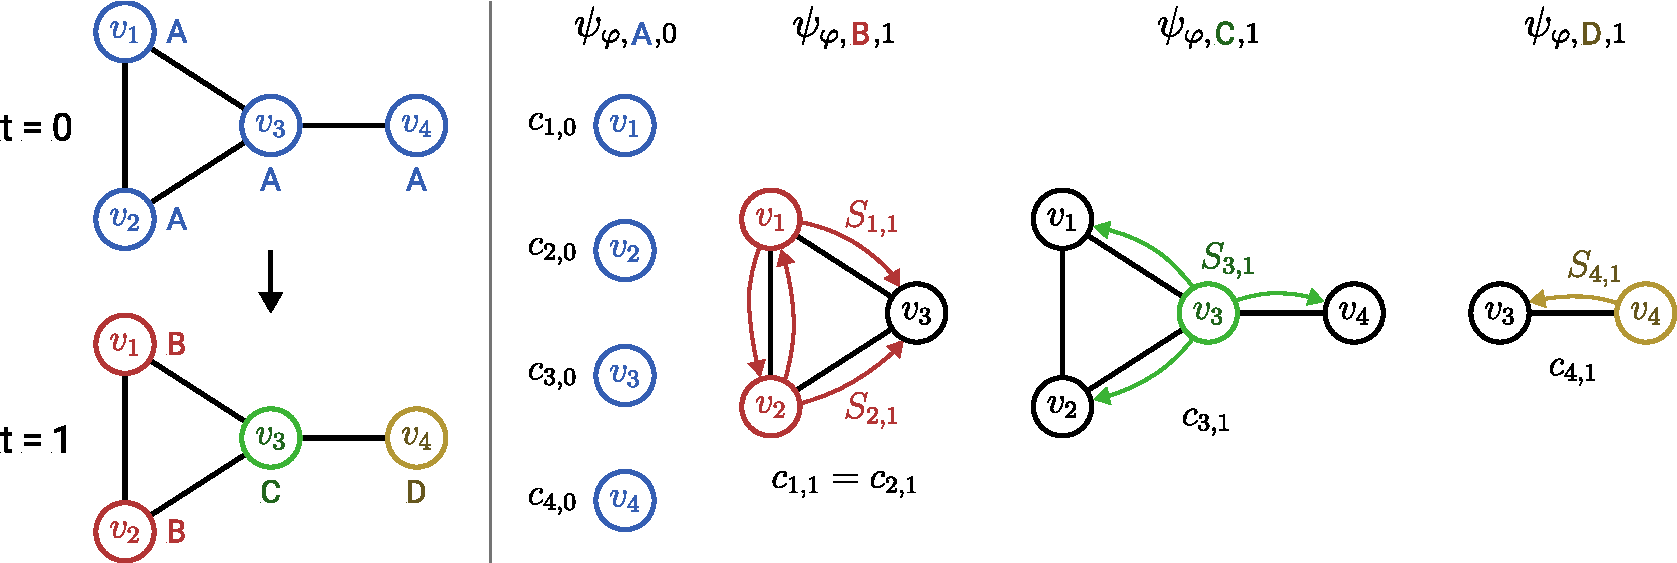
\includegraphics[width=\linewidth]{gfx/graph-lta/wl1-constituents.pdf}
			\caption[The constituents implied by the \ac{wl} subtree kernel embedding for an example graph.]{
				The constituents $c_{j,t}$ implied by the \ac{wl} subtree embedding vector $\varphi(G) = (\underbrace{\textcolor{t_blue}{4}, \textcolor{t_red}{0}, \textcolor{t_green}{0}, \textcolor{t_darkyellow}{0}}_{t = 0}, \underbrace{\textcolor{t_blue}{0}, \textcolor{t_red}{2}, \textcolor{t_green}{1}, \textcolor{t_darkyellow}{1}}_{t = 1})$. % chktex 25
				The subtrees $S_{j,t}$ that span each constituent $c_{j,t}$ are visualized by the colored arrows that originate from the colored root vertices.
				Because $S_{1,1}$ and $S_{2,1}$ span the same constituent $c = c_{1,1} = c_{2,1} = G[\{ v_1, v_2, v_3 \}]$, its multiplicity is $\gamma_{\varphi, \textcolor{t_red}{\texttt{B}}, 1}(c) = 2$; % chktex 25
				the multiplicity of all other constituents is $1$.
			}\label{fig:ltag:wl1-constituents}
		\end{figure}

		To fix the previous intuition we ``convert'' the subtrees $S_{j, t}$ into proper subgraph constituents via $c_{j,t} \coloneqq G[\mathcal{V}_{S_{j,t}}]$, i.e.\ the subgraphs that are spanned by the subtrees.
		The resulting decomposition functions are $\psi_{\varphi, i, t}(G) \coloneqq \{ c_{j,t}\, |\, {v_j \in \mathcal{V}_G}\,\land {S_{j,t} \simeq S_{\kappa_i}} \}$. % chktex 21
		As illustrated in \cref{fig:ltag:wl1-constituents}, the number of distinct constituents $c_{j,t}$ might be smaller than the number of \ac{bfs} subtrees $S_{j,t}$ because two distinct subtrees might span the same set of vertices.
		To fix this discrepancy between the subtree occurrence count (which equals $\varphi(G)[i, t]$) and the number of constituents, the multiplicities $\gamma_{\varphi, i, t}(c)$ of the constituents $c$ have to correspond to the number of \ac{bfs} subtrees they were spanned up by, i.e.\
		\begin{align}
			&\gamma_{\varphi, i, t}(c) \coloneqq {\left|\{ S = \text{\acs*{bfs}}(c, v_{\text{root}}, t)\, |\, v_{\text{root}} \in \mathcal{V}_c \land S \simeq S_{\kappa_i} \land \mathit{complete}(S) \}\right|}\label{eq:ltag:wlst-constituent-subtree-count} \\
			&\text{with }\mathit{complete}(S) \Leftrightarrow \forall\ \text{leaf nodes $v_{\text{leaf}}$ of the tree $S$}: {|\Gamma_c(v_{\text{leaf}})|} = {|\Gamma_G(v_{\text{leaf}})|}
			\text{.} \nonumber
		\end{align}
		The purpose of the $\mathit{complete}(S)$ condition is to only count the \ac{bfs} subtrees of the constituent $c$ that are also \ac{bfs} subtrees of the complete graph $G$.
		To see why this is required, note that in \cref{fig:ltag:wl1-constituents} the $c_{1,1}$/$c_{2,1}$ constituent contains the color subtree $S_{\textcolor{t_red}{\texttt{B}}}$ three times (rooted at $v_1$, $v_2$ and $v_3$) even though $G$ only contains it twice (rooted at $v_1$ and $v_2$). % chktex 25
		Also note that, since $\gamma_{\varphi, i, t}(c)$ must only depend on a given constituent $c$ and not on the graph $G$ it was decomposed from, the degree information $|\Gamma_G(v_{\text{leaf}})|$ of the constituent vertices $v \in \mathcal{V}_c$ is assumed to be statically encoded in the labels $l_c[v]$ or feature vectors $x_c[v]$.

		Via the decomposition and multiplicity functions that were just described, $\varphi_{\text{ST}}$ is in fact an \ac{sce} with a nontrivial, subtree-based decomposition function.
		Additionally each constituent's diameter is upper bounded by $2T$ (with $T$ being the maximum number of \ac{wl} iterations) which guarantees that constituents are localized within a neighborhood of bounded size.
		By \cref{thm:ltag:svm-ltag-formulation}, \acp{svm} that use the \ac{wl} subtree kernel therefore have nontrivial \ac{lta} formulations with localized constituents, i.e.\ they can be considered to be ``\ac{lta}-like'' models.
		However, unlike fingerprint embeddings, the \ac{wl} subtree constituents are not manually chosen to be interpretable.
		This implies that the localized explainability characteristic of \ac{lta} is only partially satisfied since the \ac{svm} predictions are based on local constituent predictions that are not necessarily interpretable.
		\badgebox[t_green]{\acs*{lta}-like}
	\item \textbf{\ac{wl} shortest path kernel:}\label{itm:ltag:wlsp-lta-formulation}
		As defined in \cfullref[ on ]{eq:related:wl-shortest-path-kernel}, the $i$-th component of the \ac{wl} shortest path embedding $\varphi_{\text{SP}}$ represents a 4-tuple $(t_i, a_i, b_i, d_i) \in {\{ 0, \dots, T \}} \times \mathcal{C} \times \mathcal{C} \times \mathbb{N}_0$.
		The value $\varphi_{\text{SP}}(G)[i]$ is defined as the number of vertex pairs $v_a, v_b \in \mathcal{V}_G$ that have a shortest connecting path of length $d_i$ and the \ac{wl} color combination $\chi_{G,1}^{(t_i)}(v_a) = a_i$ and $\chi_{G,1}^{(t_i)}(v_b) = b_i$.

		To determine the number of such vertex pairs via an \ac{sce} multiplicity function $\gamma_{\varphi, t_i, a_i, b_i, d_i}$, each connected pair of vertices $v_a, v_b$ and the shortest path between them must occur together in at least one constituent, otherwise a multiplicity function cannot compute whether $v_a$ and $v_b$ are in fact $d_i$ hops apart.
		One simple decomposition which guarantees that all shortest paths are part of at least one constituent simply splits a given graph into its connected components.
		Even though such a decomposition is non-trivial since it uses at least some structural information to determine the set of constituents, the fact that any pair of connected vertices must co-occur within a single constituent means that constituents must span arbitrarily large distances within a given graph.
		Depending on ones domain-specific interpretation of \textit{localized explainability}, this restriction can be seen to be not ``\acs{lta}-like''.
		Since we do not attempt to clearly separate \ac{lta} from non-\acs{lta} methods, $\varphi_{\text{SP}}$ is categorized as an in-between case here.
		\badgebox[t_yellow]{partially \acs*{lta}-like}
	\item \textbf{$k$-LWL kernel:}\label{itm:ltag:klwl-lta-formulation}
		The \ac{lta} interpretation of the $k$-LWL kernel is identical to that of the \ac{wl} subtree kernel.
		The \ac{wl} color of a $k$-multiset of vertices $s$ after $t$ refinement steps is described by the joint $t$-neighborhood of all vertices $v \in s$, i.e.\ by $\Gamma_{G}^t(s) \coloneqq \bigcup_{v \in s} \Gamma_{G}^t(v)$ where $\Gamma_{G}^t(v) \coloneqq \Gamma_{G}^{t-1}(v) \cup \bigcup_{u \in \Gamma_{G}(v)} \Gamma_{G}^{t-1}(u)$ and $\Gamma_{G}^0(v) \coloneqq \{ v \}$.
		Analogous to \ac{wl} subtree embeddings, those $t$-neighborhoods form the localized constituents of the $k$-LWL kernel via a \ac{bfs} over neighboring $k$-multisets.
		Consequently \acp{svm} using the $k$-LWL kernel can be interpreted as ``\acs{lta}-like'' methods with nontrivial localized decompositions.
		\badgebox[t_green]{\acs*{lta}-like}
	\item \textbf{$k$-GWL kernel:}\label{itm:ltag:kgwl-lta-formulation}
		The only difference between the $k$-LWL and the $k$-GWL kernel is their definition of the $k$-multiset neighborhood.
		Namely the refined color of a multiset $s \subseteq \mathcal{V}_G$ in $k$-GWL depends on the the colors of all vertices $\mathcal{V}_G$ since all multisets $s' = s \setminus \{ v \} \cup \{ u \}$ with $v \in s$ and $u \in \mathcal{V}_G$ are neighbors of $s$.
		Because of those global multiset neighborhoods, all the color subtrees of a graph span the entire graph.
		Therefore the $k$-GWL embedding is an \ac{sce} with only the trivial decomposition function $\psi_{\varphi}(G) = \{ G \}$.
		Thus the \ac{lta} formulation of $k$-GWL \acp{svm} described in \cref{thm:ltag:svm-ltag-formulation} is also trivial which means that they are not \ac{lta} models.
		\badgebox[t_red]{non-\acs*{lta}}
\end{enumerate}

This concludes our overview of \ac{lta} interpretations of \acp{svm} that use graph embeddings/kernels.
Among the described approaches, fingerprint embeddings, the \ac{wl} subtree kernel and the $k$-LWL kernel were shown to have \ac{lta} formulations with nontrivial local decomposition functions.
Approaches like \texttt{graph2vec}, the \ac{wl} shortest path kernel or $k$-GWL on the other hand, were shown to be less compatible with \ac{lta}.

\subsection{\acsp*{gcnn} as \acs*{lta} Models}%
\label{sec:ltag:formulation:gcnn}

Now we will look at \ac{gcnn} methods from an \ac{lta} perspective.
As shown in the last section, \acp{svm} can be interpreted as \ac{lta} methods if they use an \ac{sce} embedding;
similarly \acp{gcnn} also have \ac{lta} formulations under certain conditions.
In this section we will describe those conditions and the \ac{lta} formulations of the \acp{gcnn} that satisfy them.

In \cref{sec:related:gcr:nn} an overview of graph convolution and graph pooling layers was given.
While there are many ways to combine those layers, we focus on global pooling \ac{gcnn} architectures that use the following three steps:
\begin{enumerate}[label=\textbf{\arabic*.}]
	\item \textbf{Convolution:}
		First a stack of $T$ convolutional layers is applied to the input feature matrix $X \in \mathbb{R}^{n \times d^{(0)}}$ where each row is a feature vector $x_i \in \mathbb{R}^{d^{(0)}}$ for the vertex $v_i \in \mathcal{V}_G$ or the vertex $k$-multiset $s_i \subseteq \mathcal{V}_G$ in case of $k$-\acsp{gnn}.
		The convolutional layers produce a convolved feature matrix $Z \in \mathbb{R}^{n \times d^{(T)}}$ where each row is a convolved feature vector $z_i \in \mathbb{R}^{d^{(\text{pool})}}$.
	\item \textbf{Pooling:}
		Then the convolved feature matrix $Z$ is reduced to a single graph feature vector $z_G \in \mathbb{R}^{d^{(\text{pool})}}$ via a pooling layer.
	\item \textbf{\ac{mlp}:}
		Lastly the final output $y_G \in \mathcal{Y}$ is computed by applying a standard \ac{mlp} to the graph feature vector $z_G$.
\end{enumerate}
\[
	\text{\acs*{gcnn}}(G) \coloneqq \mathit{\acs*{mlp}}(\mathit{Pool}(\mathit{Conv}(G)))
\]
\Cref{fig:ltag:gcnn-structure} illustrates this three step architecture for vertex neighborhood convolutions like those used by \acp{gcn}~\cite{Kipf2017} or \acp{gin}~\cite{Xu2018}.
Intuitively the convolutional layers implicitly define an \ac{lta} decomposition function $\psi$ and a local evaluation function $f$ while the pooling layer corresponds to an \ac{lta} aggregation function $\mathcal{A}$.
This intuition is now formalized.
\begin{figure}[ht]
	\centering
	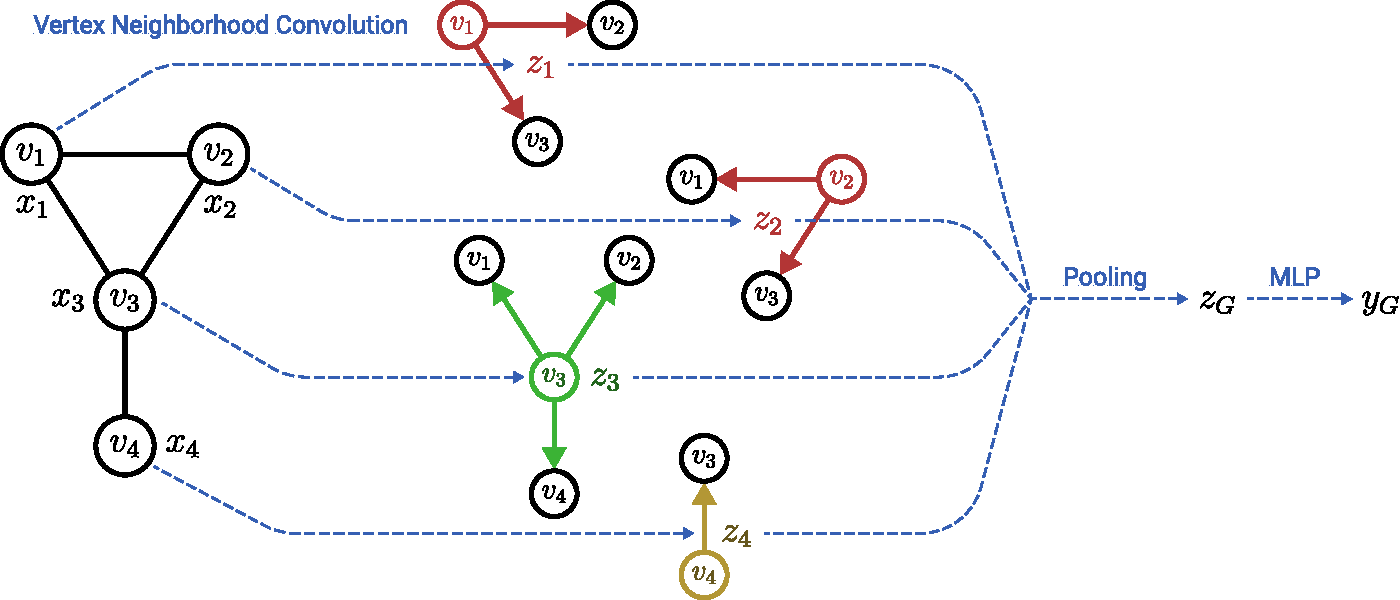
\includegraphics[width=\linewidth]{gfx/graph-lta/gcnn-structure.pdf}
	\caption[Computational steps of a \ac{gcnn} that uses a single vertex neighborhood convolution layer.]{
		Computational steps of a \ac{gcnn} that uses a single vertex neighborhood convolution layer.
		The colored \ac{bfs} trees next to each convolved feature vector $z_i$ show the vertices $v_j$ whose input feature vectors $x_j$ were used to compute $z_i$.
	}\label{fig:ltag:gcnn-structure}
\end{figure}

\subsubsection{Graph Convolutions as \ac*{lta} Decomposition and Evaluation Functions}

To define an \ac{lta} formulation for \acp{gcnn}, we define two functions that are entirely based on the stack of convolutional layers:
\begin{enumerate*}
	\item The decomposition function $\psi: \mathcal{G} \to \mathcal{P}(\mathcal{G})$.
	\item The so-called \textit{multi-score evaluation function} $f^{*}: \mathcal{G} \to {(\mathcal{Y} \times \mathbb{R}_{\geq 0})}^{*}$ which is similar to a regular \ac{lta} evaluation function $f$ but assigns a multiset of weighted scores to each constituent instead of just a single one.
\end{enumerate*}
Those two functions make up the first half of a \ac{gcnn} graph formulation.
How exactly they are defined depends on the type convolutional layer that is used.

\paragraph{Spectral convolutions with arbitrary filters}
Let us begin with general spectral graph convolutions~\cite{Bruna2013}\cite{Henaff2015}.
Following \cfullref[ on ]{eq:related:graph-conv-general}, after a single convolution the convolved feature vector $z_i$ of a vertex $v_i$ is defined as
\begin{align}\label{eq:ltag:general-spectral-conv}
	z_{\textcolor{t_red}{i}} = {\left( U^{\top} \hat{g}(\Lambda) U X \right)}_{\textcolor{t_red}{i}} % chktex 25
	= \sum_{l=1}^n u_{l,\textcolor{t_red}{i}} \hat{g}(\lambda_l) \underbrace{\sum_{j=1}^n u_{l,j} x_j}_{\mathclap{\text{$d^{(T)}$-dim.\ vector of inner products}}} % chktex 25
	= \sum_{j=1}^n \underbrace{\left( \sum_{l=1}^n \hat{g}(\lambda_l) u_{l,\textcolor{t_red}{i}} u_{l,j} \right)}_{\alpha_j} x_j % chktex 25
\end{align}
where $L = U^{\top} \Lambda U = \sum_{l=1}^n u_l \lambda_l u_l^{\top}$ is the eigendecomposition of the input graph's Laplacian and $\hat{g}$ is some (learned) eigenvalue filter.
\begin{lem}\label{lem:ltag:general-spectral-conv-nonlocality}
	For all graphs $G$ consisting of the connected components $C_1, \dots, C_m$ there is an $\eta \in \mathbb{R}$ s.t.\ if $\hat{g}(0) = \eta$, the convolved feature vector $z_i$ of each $v_i \in \mathcal{V}_{C_l}$ with $l \in [m]$ depends on all input features $x_j$ of the vertices $v_j \in \mathcal{V}_{C_l}$ from the same component.
\end{lem}
\begin{hproof}
	Note that by \cfullref[ on ]{defn:related:laplacian-comb} it follows that the first $m$ eigenvalues of a graph with the connected components $C_1, \dots, C_m$ are $\lambda_1 = \cdots = \lambda_m = 0$ with the corresponding nullspace-spanning unnormalized eigenvectors $u_l[v_j] = \mathbbm{1}[v_j \in \mathcal{V}_{C_l}]$\daggerfootnote{
		We refer to \citet{Das2004} for a more in-depth discussion of graph Laplacian eigenvectors.
	}.
	Consequently in \cref{eq:ltag:general-spectral-conv} the first $m$ summands of each $\alpha_j$ sum up to $\hat{g}(0) u_{l,j} u_{l,i} = \eta$ for all $v_i \in C_l$ with $l \in [m]$.
	The lemma then follows by choosing $\eta$ s.t.\ the last $n - m$ summands of every $\alpha_j$ do not sum up to $\eta$.
\end{hproof}
Because a \ac{gcnn} with an arbitrary learned spectral filter $\hat{g}$ can learn $\hat{g}(0) = \eta$, each convolved vertex feature vector $z_i$ potentially depends on the entire connected component $C_l$ with $v_i \in \mathcal{V}_{C_l}$.
This means that any constituent scores computed based on $z_i$ can only be computed for constituents that span entire connected components.
In other words, spectral \acp{gcnn} with arbitrary filters generally only have \ac{lta} formulations with the decomposition function $\psi(G) = \{ C_1, \dots, C_m \}$.
This restriction makes them an in-between case which is only partially \acs{lta}-like.

\paragraph{Vertex neighborhood convolutions}
Unlike spectral convolutions, spatial approaches like \acp{gcn} or \acp{gin} compute convolved feature vectors $z_i$ which only depend on the $T$-neighborhood of each vertex $v_i \in \mathcal{V}_G$.
Just like the \ac{bfs} subtree evaluations of \ac{wl} subtree kernel \acp{svm} (see \cfullref{itm:ltag:wlst-lta-formulation}), each $z_i$ can therefore be interpreted as an evaluation of a local constituent $c_i$.
As previously described, this means that two evaluations $z_i, z_j$ with $i \neq j$ are computed for a single subgraph constituent $c_i = c_j$ iff.\ the \ac{bfs} trees of $v_i$ and $v_j$ span the same vertices.
This is illustrated in \cref{fig:ltag:gcnn-structure} by \textcolor{t_red}{$z_1$} and \textcolor{t_red}{$z_2$} which are both evaluations of the constituent
$\textcolor{t_red}{c_1} = \textcolor{t_red}{c_2} = G[\{ v_1, v_2, v_3 \}]$. % chktex 25

\paragraph{Vertex $k$-multiset neighborhood convolutions}
Analogously to single vertex convolutions, the $k$-multiset convolutions of $k$-\acp{gnn} produce local evaluation vectors $z_i$ for the $T$-neighborhood of each $k$-multiset $s_i \subseteq \mathcal{V}_G$.
By \cfullref[ on ]{eq:related:kgnn-layer} the constituent $c_i$ spanned by the vertices that have an influence on $z_i$ can thus be written as $c_i = G\left[ \bigcup_{v \in s_i} \Gamma_G^T(v) \right]$.
This constituent definition is identical to that used in the \ac{lta} formulation of $k$-LWL \acp{svm} (see \cfullref{itm:ltag:klwl-lta-formulation}).

\paragraph{\ac{gcnn} \ac{lta} decomposition}
Both, the single vertex neighborhood convolution as well as the vertex $k$-multiset neighborhood convolution produce vectors $z_i \in \mathbb{R}^{d^{(T)}}$, which are each based on the constituent $c_i$ spanned by the $T$-neighborhood of some vertex $v_i$ or vertex $k$-multiset $s_i$.
Consequently we define the \ac{lta} decomposition function of such neighborhood convolution \acp{gcnn} as $\psi(G) \coloneqq {\{ c_i \}}_{i=1}^n$.

\paragraph{\ac{gcnn} \ac{lta} multi-score evaluation}
In addition to this decomposition function, the convolved vectors $z_i \in \mathbb{R}^{d^{(T)}}$ can be interpreted as local evaluations if there is a translation function $\tau_{1}: \mathbb{R}^{d^{(T)}} \to \mathcal{Y} \times \mathbb{R}_{\geq 0}$.
One trivial example for such a translation function would be the identity $\tau_{1}(z) = z$ for a graph regression problem with the score domain $\mathcal{Y} = [0, 1]$ and where the last convolutional layer uses a sigmoid activation function with two output dimensions s.t.\ $z \in {[0,1]}^2$.
Assuming that there is a translation function $\tau_{1}$ we can define a multi-score evaluation function $f^{*}(c) \coloneqq {\ldblbrace \tau_{1}(z_i)\, |\, {i \in [n]} \land {c = c_i} \rdblbrace} = {\ldblbrace \tau_{1}(\mathit{Conv}(X_c)[v_i])\, |\, v_i \in \mathit{root}(c) \rdblbrace}$ with $X_c$ being the input feature matrix of the subgraph/constituent $c$.
The function $\mathit{root}(c) = \{ v_i\, |\, {i \in [n]} \land {c = c_i} \}$ returns the set of root vertices $v_i$ (or root vertex $k$-multisets in case of $k$-\acs{gnn}) whose \ac{bfs} subtree of depth $T$ in $G$ spans exactly the vertices in $c$.
To compute $\mathit{root}(c)$ given only a single constituent $c$ and not the entire graph $G$, it has to be determined which \ac{bfs} subtrees of $c$ are also \ac{bfs} subtrees of $G$.
We already saw how to do this in the \ac{lta} formulation of \ac{wl} subtree kernel \acp{svm} (see $\mathit{complete}$ in \cfullref{eq:ltag:wlst-constituent-subtree-count}).

\subsubsection{Graph Pooling as \ac*{lta} Aggregation Functions}

Based on the decomposition function $\psi: \mathcal{G} \to \mathcal{P}(\mathcal{G})$ and the multi-score evaluation function $f^{*}: \mathcal{G} \to {(\mathcal{Y} \times \mathbb{R}_{\geq 0})}^{*}$ which are implicitly defined by the stack of convolutional layers $\mathit{Conv}$ of a given \ac{gcnn}, we now complete our \ac{gcnn} \ac{lta} formulation by defining an evaluation function $f: \mathcal{G} \to \mathcal{Y} \times \mathbb{R}_{\geq 0}$ as well as an aggregation function $\mathcal{A}: {(\mathcal{Y} \times \mathbb{R}_{\geq 0})}^{*} \to \mathcal{Y}$ based on the pooling layer $\mathit{Pool}: \mathbb{R}^{n \times d^{(T)}} \to \mathbb{R}^{d^{(\text{pool})}}$.
\begin{defn}\label{defn:ltag:assoc-algebra}
	A variadic function $\xi: A^{*} \to B$ is called \textit{variadic associative} iff.\ there is an operator $\rho: A^{*} \to A$ s.t.\ $\forall n \in \mathbb{N}: \forall (a_1, \dots, a_n) \in A^n: \forall {1 \leq i \leq j \leq n}: \xi(a_1, \dots, a_n) = \xi(a_1, \dots, a_{i-1}, \rho(a_i, \dots, a_j), a_{j+1}, \dots, a_n)$.
	The heterogeneous algebra $((A, B), (\xi, \rho))$ is called an \textit{associative algebra} of $\xi$~\cite{Birkhoff1970}.
\end{defn}
\begin{defn}[see \citet{Novotny2002}]\label{defn:ltag:assoc-algebra-homomorphism}
	A function tuple $(\tau_1: A \to C, \tau_2: B \to D)$ is a \textit{homomorphism} between two associative algebras $((A, B), (\xi, \rho))$ and $((C, D), (\xi', \rho'))$
	\begin{align*}
		\text{iff.\ }
		\forall n \in \mathbb{N}: \forall (a_1, \dots, a_n) \in A^n:
		\, &\tau_2(\xi(a_1, \dots, a_n)) = \xi'(\tau_1(a_1), \dots, \tau_1(a_n)) \\
		\land\, &\tau_1(\rho(a_1, \dots, a_n)) = \rho'(\tau_1(a_1), \dots, \tau_1(a_n)) % chktex 21
		\text{.}
	\end{align*}
\end{defn}
\begin{defn}\label{defn:ltag:assoc-aggregation-pooling}
	A pooling layer $\mathit{Pool}: \mathbb{R}^{n \times d^{(T)}} \to \mathbb{R}^{d^{(\text{pool})}}$ is called a \textit{weighted associative aggregation layer} iff.
	\begin{enumerate*}
		\item there is an associative algebra of $\mathit{Pool}$,
		\item there is a weighted aggregation function $\mathcal{A}$ with an associative algebra and
		\item there is a homomorphism $(\tau_{1}: \mathbb{R}^{d^{(T)}} \to (\mathcal{Y} \times \mathbb{R}_{\geq 0}), \tau_{2}: \mathbb{R}^{d^{(\text{pool})}} \to \mathcal{Y})$ from the associative algebra of $\mathit{Pool}$ to that of $\mathcal{A}$
	\end{enumerate*}.
\end{defn}
Using those definitions we can complete the connection between \acp{gcnn} and \ac{lta}:
\begin{thm}\label{thm:ltag:gcnn-ltag-formulation}
	A \ac{gcnn} of the form $\mathit{Pool}(\mathit{Conv}(X_G))$ has a nontrivial \ac{lta} formulation if $\mathit{Conv}$ is a stack of neighborhood convolutions and $\mathit{Pool}$ is a weighted associative aggregation layer.
\end{thm}
\begin{proof}
	We already saw that the stack of neighborhood convolutions computes the values of a multi-score evaluation function $f^{*}$ for the subtree constituents returned by a decomposition function $\psi$.
	Since $\mathit{Pool}$ is assumed to be a weighted associative aggregation layer, there must be an operator $\rho_{\mathit{Pool}}: \mathbb{R}^{n \times d^{(T)}} \to \mathbb{R}^{n \times d^{(T)}}$ and a homomorphism $(\tau_{1}, \tau_{2})$ to an associative algebra with the operators $\mathcal{A}: {(\mathcal{Y} \times \mathbb{R}_{\geq 0})}^{*} \to \mathcal{Y}$ and $\rho_{\mathcal{A}}: {(\mathcal{Y} \times \mathbb{R}_{\geq 0})}^{*} \to {(\mathcal{Y} \times \mathbb{R}_{\geq 0})}$.
	This allows us to rewrite the \ac{gcnn} as
	\begin{align*}
		\tau_2(\mathit{Pool}(\mathit{Conv}(X_G)))
		&= \tau_2(\mathit{Pool}(\ldblbrace z_i\, |\, z_i = \mathit{Conv}(X_G)[v_i] \land v_i \in \mathcal{V}_G \rdblbrace)) \\
		&= \tau_2(\mathit{Pool}(\ldblbrace \mathit{Conv}(X_c)[v_i]\, |\, c \in \psi(G) \land v_i \in \mathit{root}(c) \rdblbrace)) \\
		&= \tau_2(\mathit{Pool}(\ldblbrace \rho_{\mathit{Pool}}(\ldblbrace \mathit{Conv}(X_c)[v_i]\, |\, v_i \in \mathit{root}(c) \rdblbrace)\, |\, c \in \psi(G) \rdblbrace)) \\
		&= \mathcal{A}(\ldblbrace \rho_{\mathcal{A}}(\ldblbrace \tau_1(\mathit{Conv}(X_c)[v_i])\, |\, v_i \in \mathit{root}(c) \rdblbrace)\, |\, c \in \psi(G) \rdblbrace) \\
		&= \mathcal{A}(\ldblbrace \underbrace{\rho_{\mathcal{A}}(f^{*}(c))}_{f(c)}\, |\, c \in \psi(G) \rdblbrace)
		= \mathcal{A}(\ldblbrace f(c)\, |\, c \in \psi(G) \rdblbrace)
		\text{.}
	\end{align*}
	The \ac{lta} formulation above is for vertex neighborhood convolutions;
	a formulation for vertex $k$-multiset neighborhood convolutions can be obtained analogously which concludes the proof\footnote{
		Note that the \ac{lta} formulation in this proof assumes that the \ac{gcnn}'s output is translated into the target score space via $\tau_{2}: \mathbb{R}^{d} \to \mathcal{Y}$, e.g.\ if the \ac{gcnn} returns one-hot vector encodings of discrete classes $y \in \mathcal{Y}$ those must be decoded.
	}.
\end{proof}
Note that \cref{thm:ltag:gcnn-ltag-formulation} requires \acp{gcnn} without the final \ac{mlp} proposed in the \ac{gcn}~\cite{Kipf2017} and \gc{gin}~\cite{Xu2018} papers (see \cref{fig:ltag:gcnn-structure}).
The reason for this is that the composition $\mathit{\acs*{mlp}} \circ \mathit{Pool}$ cannot be guaranteed to be homomorphic to a weighted aggregation function $\mathcal{A}$ due to the universal approximation theorem.

Lastly we will see which graph pooling layers satisfy \cref{defn:ltag:assoc-aggregation-pooling} and are therefore allowed in \ac{lta} \acp{gcnn}.


\section{A Novel \acs*{lta}-Inspired \acs*{gcnn} Architecture}%
\label{sec:ltag:wl2gnn}

\subsection{Shortcomings of $k$-\acsp*{gnn}}%
\label{sec:ltag:wl2gnn:kgnn-problems}

\subsection{The 2-\acs*{wl} Convolution Operator}%
\label{sec:ltag:wl2gnn:definition}

\subsection{The Expressive Power of 2-\acs*{wl}-\acsp*{gcnn}}%
\label{sec:ltag:wl2gnn:properties}

\subsection{Efficient Implementation on \acsp*{gpgpu}}%
\label{sec:ltag:wl2gnn:implementation}
